\documentclass[10pt,conference]{IEEEtran}
\IEEEoverridecommandlockouts

\usepackage{cite}
\usepackage{amsmath,amssymb,amsfonts}
\usepackage{graphicx}
\usepackage{textcomp}
\usepackage{xcolor}
\usepackage{booktabs}
\usepackage{url}
\usepackage{balance}
\usepackage{tikz}
\usepackage{pgfplots}
\usetikzlibrary{positioning,shapes.geometric,arrows.meta}
\pgfplotsset{compat=1.18}

\setlength{\textfloatsep}{3.8pt plus 1pt minus 1pt}
\setlength{\floatsep}{3.8pt plus 1pt minus 1pt}
\setlength{\intextsep}{3.8pt plus 1pt minus 1pt}
\setlength{\abovecaptionskip}{2pt plus 1pt minus 1pt}
\setlength{\belowcaptionskip}{1pt plus 1pt minus 1pt}

\begin{document}

\title{BR-Bench: A Benchmark Linking Continuous Integration Changes to Fault-Revealing Tests}

\author{
\IEEEauthorblockN{Deepanshu\IEEEauthorrefmark{1}, Sanskriti Singh\IEEEauthorrefmark{1}, Prisha Vadhavkar\IEEEauthorrefmark{1}, Dr.~Yoga Raja C A\IEEEauthorrefmark{2}}
\IEEEauthorblockA{\IEEEauthorrefmark{1}School of Computer Science Engineering and Information Systems\\
Vellore Institute of Technology, Vellore, Tamil Nadu, India\\
\{deepanshu.2023, sanskriti.singh2023, prisha.vadhavkar2023\}@vitstudent.ac.in}
\IEEEauthorblockA{\IEEEauthorrefmark{2}Assistant Professor Sr. Grade 1, Department of Information Technology\\
School of Computer Science Engineering and Information Systems\\
Vellore Institute of Technology, Vellore, Tamil Nadu, India\\
yogaraja.ca@vit.ac.in}
}

\maketitle

\begin{abstract}
\textsc{BR-Bench} is a dataset that links pull-request changes to the individual tests they cause to fail in continuous integration (CI). We mined GitHub Actions runs of Java and Python repositories, parsed test verdicts out of Maven, Gradle and pytest job logs, and paired each failing head run with a base run (a run of the same workflow on the branch the pull request targets). A test is fault-revealing if it fails at the head, does not fail in the base run, and does not flip between runs of one commit. The strict split holds 762 failing runs with 4,168 fault-revealing labels on 2,466 distinct tests from 37 repositories. Of 5,985 test identifiers, 5,643 (94.29\%) bind to a source file in a pinned clone, and 3,820 (63.83\%) bind at full confidence. As one use of the data we compare cheap proxies for the tests a change breaks; at $k=10$, failure history recalls 39.44\% of the fault-revealing test files and file co-change 4.64\%. No language model takes part in the pipeline, and one offline command regenerates the reported numbers.
\end{abstract}

\begin{IEEEkeywords}
continuous integration, test selection, regression testing, mining software repositories, fault revelation
\end{IEEEkeywords}

\section{Introduction}

\textsc{BR-Bench} is a dataset of CI runs in which every failing pull-request run is linked to the tests that the change caused to fail. We call these tests fault-revealing (tests that fail at the head commit, do not fail in the matching base run, and give the same verdict in every run of one commit). The labels come from what GitHub Actions actually executed in 76 repositories, not from a static model of the code.

The underlying question is short. Given a diff, which tests will fail? At Meta the answer comes from a model trained on internal test logs, see Machalica et al.~\cite{machalica2019predictive}, and Memon et al.~\cite{memon2017taming} describe how large the problem is at Google; neither body of data is public. Regression test selection takes another route. Tools such as Ekstazi~\cite{gligoric2015practical} and STARTS~\cite{legunsen2017starts} compute, from file or class dependencies, a safe superset of the tests a change may affect. Change impact analysis usually asks which entities are edited together, often from version history~\cite{borg2017supporting,huang2022change}; that is a statement about editing, not about failure. Public CI datasets stop before the test level of a single change (Section~\ref{sec:related}).

Three things make the labels hard to obtain. GitHub Actions keeps test output only as free text, so verdicts must be parsed. A test that fails at the head may already fail at the base. And some tests are flaky. We answer the first with deterministic parsers, the second with base-run resolution, and the third with a filter on same-commit flips.

\textit{Summary of results.}
\begin{itemize}
\item The strict split has 762 instances, 4,168 labels and 2,466 distinct tests from 37 repositories (Section~\ref{sec:overview}, Table~\ref{tab:splits}).
\item 94.29\% of test identifiers bind to a file, 63.83\% at full confidence (Table~\ref{tab:quality}).
\item 43.88\% of failed runs have no usable base run, and 0.54\% of test groups flip on one commit (Section~\ref{sec:collection}).
\item At $k=10$, failure history recalls 39.44\% of fault-revealing test files and co-change 4.64\% (Section~\ref{sec:rq1}, Fig.~\ref{fig:rq1}).
\item The release misses the 5,000-label target and the full-confidence binding target we set ourselves (Section~\ref{sec:limits}).
\end{itemize}

\section{Data Source and Collection}
\label{sec:collection}

\begin{figure}[t]
\centering
%
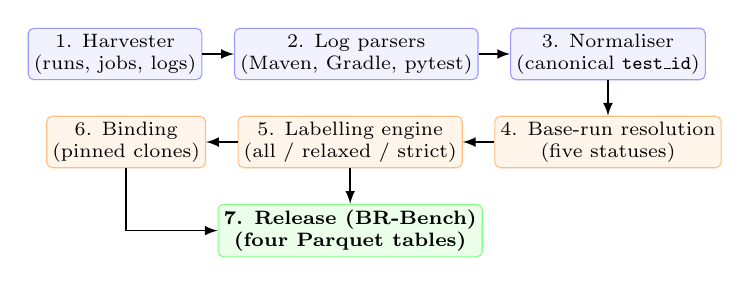
\begin{tikzpicture}[
  node distance=0.45cm and 0.4cm,
  every text node part/.style={align=center},
  box/.style={draw, rectangle, rounded corners=2pt, minimum height=0.6cm, minimum width=1.1cm, font=\scriptsize, inner sep=2pt, fill=black!4},
  proc/.style={box, fill=blue!5, draw=blue!40},
  filter/.style={box, fill=orange!8, draw=orange!50},
  res/.style={box, fill=green!8, draw=green!50, font=\scriptsize\bfseries},
  arr/.style={->, >=latex, semithick}
]
  \node[proc] (harvest) {1. Harvester\\(runs, jobs, logs)};
  \node[proc, right=of harvest] (parse) {2. Log parsers\\(Maven, Gradle, pytest)};
  \node[proc, right=of parse] (norm) {3. Normaliser\\(canonical \texttt{test\_id})};
  \node[filter, below=of norm] (base) {4. Base-run resolution\\(five statuses)};
  \node[filter, left=of base] (label) {5. Labelling engine\\(all / relaxed / strict)};
  \node[filter, left=of label] (bind) {6. Binding\\(pinned clones)};
  \node[res, below=of label] (release) {7. Release (\textsc{BR-Bench})\\(four Parquet tables)};

  \draw[arr] (harvest) -- (parse);
  \draw[arr] (parse) -- (norm);
  \draw[arr] (norm) -- (base);
  \draw[arr] (base) -- (label);
  \draw[arr] (label) -- (bind);
  \draw[arr] (bind) |- (release);
  \draw[arr] (label) -- (release);
\end{tikzpicture}%

\caption{The seven stages that turn GitHub Actions runs into the \textsc{BR-Bench} tables.}
\label{fig:pipeline}
\end{figure}

The harvester, the parsers and the labelling engine form a pipeline of seven stages (Fig.~\ref{fig:pipeline}). We take them in order.

\textit{Repository sampling.} Candidates come from the SEART search tool for GitHub, as described by Dabi\'c et al.~\cite{dabic2021sampling}. Of 3,671 exported repositories, 2,646 had at least 100 GitHub Actions runs in the 90 days before export, and 2,333 of these had a workflow that runs tests rather than only linting or deployment. We drew 300 of them, balanced between Java and Python, into a sampling frame. The harvester ran from 8 to 29 August 2026 and reached 77 repositories with 175,038 runs; the instance table covers 76 of them and 165,349 runs. For each run it stored run and job metadata, check-run annotations and the raw logs, all through the GitHub REST API.

\textit{Log parsing.} Deterministic line parsers read Maven Surefire and Failsafe, Gradle and pytest output and emit, for each test, a verdict (pass, fail, error or skip) and a duration where the log prints one. Each test then gets a canonical identifier, the \texttt{test\_id}. We write Java tests as \texttt{fully.qualified.Class\#method} and Python tests as \texttt{path::name}. If a log names only a bare class, we recover its package from other lines of the same log where we can.

\textit{Base-run resolution.} Let $H$ be the head commit of a failed pull-request run and $B$ the commit of the target branch. A base run is a run of the same workflow that tells us which tests already failed without the change. We search for one in a fixed order and record which case applied: \texttt{exact\_green} (a successful base run whose log shows that tests ran and none failed, so the base failure set is empty), \texttt{exact} (another run on $B$), \texttt{ancestor} (a run on an ancestor of $B$ at most 10 commits away), \texttt{branch\_prior} (the latest run on the target branch that started before the head run) or \texttt{no\_base}. A successful run whose log does not show tests running counts as no base at all, and a run with \texttt{no\_base} yields no label. Of the 12,581 failed runs, 5,520 (43.88\%) end as \texttt{no\_base}. Among the 6,025 resolved runs with a recorded distance, the median is 0 commits, the 90th percentile 2 and the maximum 10.

\textit{Labels and splits.} We write $F_H$ for the set of tests that fail in a head run, $F_B$ for the set that fail in its base run, and $X$ for the same-SHA flips (tests that fail in some, but not all, runs of one workflow on one commit). The fault-revealing set is
\begin{equation}
T_{\text{reveal}} = (F_H \setminus F_B) \setminus X .
\end{equation}
The labelling engine emits three nested splits. The \texttt{all} split holds every head failure in a run with a usable base and parsed head output; \texttt{relaxed} removes $F_B$; \texttt{strict} also removes $X$. A test is flaky if its verdict changes while the code does not, see Bell et al.~\cite{bell2018deflaker}, and same-SHA flips are the form of flakiness our data can observe. Flips are rare. They occur in 62 of 11,557 (head SHA, workflow, test) groups (0.54\%) and remove 46 of 4,214 relaxed labels (1.09\%).

\textit{Binding.} A label is more useful when it names a file. We bind each \texttt{test\_id} to a test source file inside a clone pinned to a recorded commit, never to a moving branch head, so the result does not depend on when a machine last fetched. A unique match on the fully qualified class name has confidence 1.0; a match on the bare class name has confidence 0.5.

\section{Storage and Schema}
\label{sec:schema}

\begin{table}[t]
\caption{Main Fields of the \textsc{BR-Bench} Tables (Release v0.2)}
\label{tab:schemas}
\centering
\scriptsize
\setlength{\tabcolsep}{2pt}
\renewcommand{\arraystretch}{0.90}
\begin{tabular}{@{}lp{4.9cm}@{}}
\toprule
\textbf{Field} & \textbf{Content} \\
\midrule
\multicolumn{2}{@{}l}{\textit{\textbf{instances} (165,349 rows; one per workflow run)}} \\
\texttt{instance\_id} & key; SHA-256 of repository, head SHA and run id \\
\texttt{repo}, \texttt{language} & \texttt{owner/name}; Java or Python \\
\texttt{head\_sha}, \texttt{base\_sha} & head commit; target-branch commit \\
\texttt{run\_started\_at} & UTC start time, typed timestamp \\
\texttt{base\_run\_id} & resolved base run \\
\texttt{base\_status} & one of the five statuses, or \texttt{not\_attempted} \\
\texttt{base\_run\_distance} & commits between base run and $B$ (at most 10) \\
changeset fields & \texttt{n\_files\_changed}, \texttt{n\_lines\_changed}, \texttt{touches\_*}, \texttt{is\_docs\_only}, \texttt{changed\_files}; null without a diff \\
\texttt{author\_login} & keyed hash, 16 hex characters \\
\midrule
\multicolumn{2}{@{}l}{\textit{\textbf{outcomes} (12,766 rows; one per run, test and split)}} \\
\texttt{run\_id}, \texttt{test\_id} & run key; canonical test identifier \\
\texttt{split} & \texttt{all}, \texttt{relaxed} or \texttt{strict} \\
\texttt{test\_file}, \texttt{binding\_*} & bound source path; binding status and confidence \\
\texttt{status\_head} & head verdict (fail or error) \\
\texttt{n\_job\_rows} & matrix legs merged into the row \\
\texttt{duration\_s} & test duration in seconds \\
\texttt{failure\_message\_hash} & SHA-256 of the failure text \\
\midrule
\multicolumn{2}{@{}l}{\textit{\textbf{cochange} (175,204 rows)}: \texttt{file\_a}, \texttt{file\_b}, \texttt{support}, \texttt{lift}, \texttt{conf\_*}} \\
\multicolumn{2}{@{}l}{\textit{\textbf{failure\_messages} (3,490 rows)}: \texttt{run\_id}, \texttt{job\_id}, \texttt{test\_id}, \texttt{failure\_message}} \\
\bottomrule
\end{tabular}
\end{table}

\textsc{BR-Bench} consists of four Apache Parquet tables, documented by a datasheet in the form proposed by Gebru et al.~\cite{gebru2021datasheets}. Table~\ref{tab:schemas} lists their main fields. The \texttt{instances} table has one row per workflow run. The \texttt{outcomes} table has one row per (run, test, split) triple, over 4,384 distinct run and test pairs. The \texttt{cochange} table holds pairs of files edited in the same commit, with support, lift and confidence in both directions, and \texttt{failure\_messages} holds the failure text recorded for a labelled test. Every count in this section can be read directly from the release files.

\textit{Releases.} Release v0.1 is published on Zenodo~\cite{brbench_data}. Release v0.2 is built and validated against its schema locally; it is not yet deposited. It keeps the four tables and their row counts and adds fields. In \texttt{instances} these are \texttt{base\_run\_id} (filled for 7,061 runs), \texttt{base\_status}, \texttt{base\_run\_distance} (filled for 6,025 runs), a typed \texttt{run\_started\_at}, and the changeset fields, which are null for the 17,364 runs without a recorded diff. In \texttt{outcomes} they are \texttt{test\_file} (4,229 of 4,384 pairs, 96.5\%), the binding status and confidence, \texttt{n\_job\_rows} (above 1 for 690 pairs, i.e., tests that ran in several matrix legs), \texttt{duration\_s} (2,505 pairs, 57.1\%) and the failure-message hash (2,111 pairs, 48.2\%).

\textit{Privacy.} We replace each author login with an HMAC-SHA256 hash under a key the operator holds, truncated to 16 hex characters; the release has 1,791 distinct hashed authors. A secret scan runs before every release. For v0.1 it found no blocking secret, and the authors checked each finding it flagged for review by hand. The findings flagged in v0.2 still await that check, which is one reason v0.2 is not yet deposited.

\section{Dataset Overview and Quality}
\label{sec:overview}

\begin{table}[t]
\caption{Attrition of Repositories and Runs Through the Pipeline}
\label{tab:funnel}
\centering
\scriptsize
\setlength{\tabcolsep}{3pt}
\renewcommand{\arraystretch}{0.90}
\begin{tabular}{@{}lrrr@{}}
\toprule
\textbf{Stage} & \textbf{Count} & \textbf{\% of prev.} & \textbf{\% of first} \\
\midrule
\multicolumn{4}{l}{\textit{Repositories}} \\
Exported from SEART & 3,671 & -- & 100.00\% \\
$\ge 100$ runs in 90 days & 2,646 & 72.08\% & 72.08\% \\
Has a test workflow & 2,333 & 88.17\% & 63.55\% \\
In the sampling frame & 300 & 12.86\% & 8.17\% \\
Reached by the harvester & 76 & 25.33\% & 2.07\% \\
Has a failed run & 69 & 90.79\% & 1.88\% \\
Has a strict instance & 37 & 53.62\% & 1.01\% \\
\midrule
\multicolumn{4}{l}{\textit{Workflow runs}} \\
Discovered & 165,349 & -- & 100.00\% \\
Failed & 12,581 & 7.61\% & 7.61\% \\
Failed-job log on disk & 6,586 & 52.35\% & 3.98\% \\
At least one parsed failing test & 1,774 & 26.94\% & 1.07\% \\
Base run resolved & 1,348 & 75.99\% & 0.82\% \\
Base failure set known & 897 & 66.54\% & 0.54\% \\
At least one strict label & 762 & 84.95\% & 0.46\% \\
\bottomrule
\end{tabular}
\end{table}

\textit{Attrition.} Table~\ref{tab:funnel} follows repositories and runs through the pipeline. The largest losses occur at the logs. Of the 12,581 failed runs, 6,586 (52.35\%) have a failed-job log on disk, and only 1,774 of these contain a failing test that the parsers recognise. A base run is found for 1,348 of them. For 897 the base failure set is known, either because the base run was \texttt{exact\_green} or because its log was parsed, and 762 keep at least one strict label.

\begin{table}[t]
\caption{Splits by Size and Language}
\label{tab:splits}
\centering
\scriptsize
\setlength{\tabcolsep}{3pt}
\renewcommand{\arraystretch}{0.90}
\begin{tabular}{@{}lrrrrr@{}}
\toprule
\textbf{Split} & \textbf{Inst.} & \textbf{Labels} & \textbf{Tests} & \textbf{Java inst.} & \textbf{Python inst.} \\
\midrule
\texttt{all} & 897 & 4,384 & 2,500 & 767 (85.5\%) & 130 (14.5\%) \\
\texttt{relaxed} & 770 & 4,214 & 2,484 & 646 (83.9\%) & 124 (16.1\%) \\
\texttt{strict} & 762 & 4,168 & 2,466 & 638 (83.7\%) & 124 (16.3\%) \\
\bottomrule
\end{tabular}
\end{table}

\textit{Composition.} Table~\ref{tab:splits} gives the size of each split. Java dominates. It accounts for 638 of the 762 strict instances (83.73\%), 3,855 of the 4,168 strict labels (92.49\%) and 35 of the 37 repositories; Python contributes 124 instances and 313 labels from 2 repositories.

\begin{table}[t]
\caption{Binding of Test Identifiers and Classes of Failure}
\label{tab:quality}
\centering
\scriptsize
\setlength{\tabcolsep}{3pt}
\renewcommand{\arraystretch}{0.90}
\begin{tabular}{@{}lrr@{}}
\toprule
\textbf{Measure} & \textbf{Count} & \textbf{Share} \\
\midrule
\multicolumn{3}{l}{\textit{Binding, over 5,985 (repository, \texttt{test\_id}) pairs}} \\
Fully qualified class name, $c=1.0$ & 3,820 & 63.83\% \\
Bare class name only, $c=0.5$ & 1,823 & 30.46\% \\
\textbf{Bound in total} & \textbf{5,643} & \textbf{94.29\%} \\
Not in the pinned tree & 178 & 2.97\% \\
Several matching files & 164 & 2.74\% \\
\midrule
\multicolumn{3}{l}{\textit{Failure class, over 4,168 strict labels}} \\
Code-level assertion & 729 & 17.49\% \\
Timeout & 112 & 2.69\% \\
Environment (GPU, network, service) & 89 & 2.14\% \\
Unknown & 3,238 & 77.69\% \\
\bottomrule
\end{tabular}
\end{table}

\textit{Binding and failure classes.} Table~\ref{tab:quality} reports binding over 5,985 distinct (repository, \texttt{test\_id}) pairs. Of these, 5,643 (94.29\%) bind to a file, 3,820 by fully qualified class name and 1,823 by bare class name. The other 342 are either absent from the pinned tree (178) or match several files (164). We also sort the failure message of each strict label into classes with an ordered list of regular expressions. The result is a lower bound on environment failures, because a label without a recorded message counts as unknown. Of the 3,238 unknown labels, 2,231 have no recorded message at all.

\section{How the Data Has Been Used: RQ1}
\label{sec:rq1}

\begin{figure}[t]
\centering
\vspace{-4pt}
\resizebox{0.65\columnwidth}{!}{%
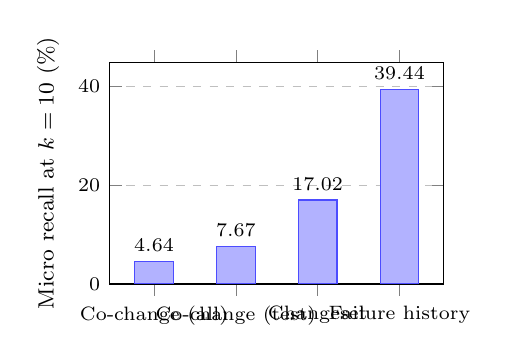
\begin{tikzpicture}
\begin{axis}[
    ybar,
    bar width=14pt,
    width=0.48\textwidth,
    height=4.4cm,
    ymin=0,
    ymax=45,
    ylabel={Micro recall at $k=10$ (\%)},
    symbolic x coords={Co-change (all), Co-change (test), Changeset, Failure history},
    xtick=data,
    nodes near coords,
    nodes near coords align={vertical},
    every node near coord/.append style={font=\scriptsize},
    tick label style={font=\scriptsize},
    label style={font=\footnotesize},
    ymajorgrids=true,
    grid style=dashed,
    enlarge x limits=0.18,
]
\addplot[fill=blue!30, draw=blue!70] coordinates {
    (Co-change (all), 4.64)
    (Co-change (test), 7.67)
    (Changeset, 17.02)
    (Failure history, 39.44)
};
\end{axis}
\end{tikzpicture}%
}
\vspace{-6pt}
\caption{Micro recall at $k=10$ of four proxies on the same 576 strict instances (1,316 fault-revealing test files).}
\label{fig:rq1}
\vspace{-6pt}
\end{figure}

We use the data to ask one question. \textit{RQ1: how well do cheap proxies for change impact find the fault-revealing test files of a change?}

\textit{Methods.} Each method returns at most $k$ test files for an instance. Co-change (all) returns the files edited together with the changed files most often, counted over the 365 days of commits before the run started (support at least 2). Co-change (test) keeps only conventional test files (paths under \texttt{src/test/}, names such as \texttt{*Test.java} or \texttt{test\_*.py}). The changeset baseline returns the changed files themselves. Failure history returns the $k$ test files with the most strict labels in runs that started earlier, each (test, run) counted once.

\textit{Leakage.} An earlier version of this measurement saw the future. A static co-change table, mined at the end of the harvest, contained commits made after the run in all 713 audited instances, and in 640 of them such a commit touched a changed file. The failure-history baseline counted labels from all three splits (224,758 rows for 78,399 distinct labels). With trailing windows, lookups in both directions of a file pair, and one count per strict label, the audit finds no violation (0 of 713 co-change instances, 0 of 762 failure-history instances).

\textit{Results.} Of the 734 strict instances with at least one bound label, 576 have a non-empty co-change set (462 Java, 114 Python), and we score every method on exactly these, with 1,316 fault-revealing test files. Fig.~\ref{fig:rq1} shows micro recall at $k=10$. Co-change (all) finds 61 of the 1,316 files (4.64\%) and co-change (test) 101 (7.67\%). The changeset baseline finds 224 (17.02\%) and failure history 519 (39.44\%). The order does not change when environment and timeout labels are removed. Co-change is a poor proxy for the tests a change breaks. Failure history needs no analysis of the code at all, and on these data it is the baseline to beat.

\section{Originality and Related Datasets}
\label{sec:related}

\textit{CI datasets.} The closest public dataset is RTPTorrent~\cite{mattis2020rtptorrent}. Its unit is a Travis CI build job of a Java project and its target use is test prioritisation, so it does not tie a diff to the tests that the diff broke. GHALogs~\cite{moriconi2025ghalogs} holds far more GitHub Actions logs than we do, but stores them unprocessed; a user still has to parse tests, find base runs and remove flaky tests. \textsc{BR-Bench} performs those three steps and publishes the result.

\textit{Selection and impact tools.} Ekstazi~\cite{gligoric2015practical} tracks file dependencies at run time, STARTS~\cite{legunsen2017starts} computes class dependencies statically, and Chianti~\cite{ren2004chianti} splits a change into atomic edits and finds the tests each one affects. These tools aim at safety (no affected test is skipped); \textsc{BR-Bench} records which tests did fail. The two views fit together, since our labels could measure how much larger a safe selection is than the set of tests that matter.

\textit{Industrial studies.} The predictive selection system of Machalica et al.~\cite{machalica2019predictive} and the Google study of Memon et al.~\cite{memon2017taming} rest on internal monorepos whose data are not released.

\section{Limitations and Threats}
\label{sec:limits}

\textit{Gates not met.} Before collection we set two targets, Gate~1 (at least 5,000 strict labels) and Gate~1.5 (at least 70\% binding). The release reaches 4,168 labels, 83.36\% of the target, and 762 instances, 15.24\% of the same figure read as instances. Gate~1.5 is met on combined binding (94.29\%) and not met at full confidence (63.83\%).

\textit{Parser precision.} The parsers score 46 of 46 on the fixture corpus and 30 of 30 on holdout v1, but both sets guided development, so these are fit figures, not held-out precision. An independent holdout (v5) exists and is not scored, because no blind human annotation was completed.

\textit{Observational labels.} We re-ran no test. A label says that a test failed in CI at the head and not at the base; it does not prove that the change caused the failure. Environment failures and timeouts remain in the strict split.

\textit{Log expiry.} GitHub Actions deletes logs after 90 days. At the last capture (29 August 2026), 4,458 of the 13,422 failed runs in the harvest corpus (33.21\%) were already older than that, so a fresh harvest cannot rebuild the dataset. Rebuilding the labels from logs needs our raw log store, which the Zenodo bundle does not contain.

\textit{Skew.} 35 of the 37 strict repositories are Java projects, and a small number of active repositories contribute a large share of the instances.

\section{Future Research Questions}

The data suggest three directions. (1)~\textit{Learned selection:} train rankers on diffs and failure history and compare them with failure history alone under a chronological split. (2)~\textit{Re-execution:} re-run head and base in containers to separate regressions from environment failures. (3)~\textit{Coverage:} add further languages and test runners. The repository also contains a ranking benchmark and a repair benchmark built on \textsc{BR-Bench}; this paper does not report them.

\section{Availability and Reproducibility}

The code is released under the MIT licence and the tables under CC BY 4.0; the mined repositories keep their own licences. Release v0.1, with \texttt{instances}, \texttt{outcomes}, \texttt{cochange} and \texttt{failure\_messages}, is on Zenodo~\cite{brbench_data} (DOI 10.5281/zenodo.23250262), and the code is archived there as well~\cite{brbench_code} (DOI 10.5281/zenodo.23250690). Release v0.2 is built and validated locally and is not yet deposited. Every number outside Section~\ref{sec:schema} regenerates offline with \texttt{make tables} (\texttt{BR\_OFFLINE=1}); the counts in Section~\ref{sec:schema} are read from the release files. The artefact's own test suite has 1,041 tests; under \texttt{make test}, 1,039 pass and 2 are skipped.

\section{Concluding Remarks}

\textsc{BR-Bench} links pull-request changes to the tests they broke in real CI runs, after removing failures inherited from the base and failures that flip on one commit. Two questions stay open. How many strict labels would survive an isolated re-run? And does any signal drawn from the code add to failure history once both are measured on the same labels? We hope the data make both questions testable.

\section*{Acknowledgment}
Generative AI assistants (Google Antigravity and Anthropic Claude) helped draft and edit parts of the text, check references and develop the artefact's software. The authors reviewed, rewrote and checked all content. No AI system takes part in data collection, labelling or the computation of any reported number; every number regenerates from the artefact through \texttt{make tables} and the release files.

\clearpage
\balance
% Generated by IEEEtran.bst, version: 1.14 (2015/08/26)
\begin{thebibliography}{10}
\providecommand{\url}[1]{#1}
\csname url@samestyle\endcsname
\providecommand{\newblock}{\relax}
\providecommand{\bibinfo}[2]{#2}
\providecommand{\BIBentrySTDinterwordspacing}{\spaceskip=0pt\relax}
\providecommand{\BIBentryALTinterwordstretchfactor}{4}
\providecommand{\BIBentryALTinterwordspacing}{\spaceskip=\fontdimen2\font plus
\BIBentryALTinterwordstretchfactor\fontdimen3\font minus
  \fontdimen4\font\relax}
\providecommand{\BIBforeignlanguage}[2]{{%
\expandafter\ifx\csname l@#1\endcsname\relax
\typeout{** WARNING: IEEEtran.bst: No hyphenation pattern has been}%
\typeout{** loaded for the language `#1'. Using the pattern for}%
\typeout{** the default language instead.}%
\else
\language=\csname l@#1\endcsname
\fi
#2}}
\providecommand{\BIBdecl}{\relax}
\BIBdecl

\bibitem{machalica2019predictive}
M.~Machalica, A.~Samylkin, M.~Porth, and S.~Chandra, ``Predictive test
  selection,'' in \emph{Proc. 41st Int. Conf. Softw. Eng.: Softw. Eng. Pract.
  (ICSE-SEIP)}.\hskip 1em plus 0.5em minus 0.4em\relax IEEE, 2019, pp. 91--100.

\bibitem{memon2017taming}
A.~Memon, Z.~Gao, B.~Nguyen, S.~Dhanda, E.~Nickell, R.~Siemborski, and
  J.~Micco, ``Taming {Google}-scale continuous testing,'' in \emph{Proc. 39th
  Int. Conf. Softw. Eng.: Softw. Eng. Pract. (ICSE-SEIP)}.\hskip 1em plus 0.5em
  minus 0.4em\relax IEEE, 2017, pp. 233--242.

\bibitem{gligoric2015practical}
M.~Gligoric, L.~Eloussi, and D.~Marinov, ``Practical regression test selection
  with dynamic file dependencies,'' in \emph{Proc. 2015 Int. Symp. Softw. Test.
  Anal. (ISSTA)}.\hskip 1em plus 0.5em minus 0.4em\relax ACM, 2015, pp.
  211--222.

\bibitem{legunsen2017starts}
O.~Legunsen, A.~Shi, and D.~Marinov, ``{STARTS}: {STAtic} regression test
  selection,'' in \emph{Proc. 32nd IEEE/ACM Int. Conf. Automated Softw. Eng.
  (ASE), Tool Demos}.\hskip 1em plus 0.5em minus 0.4em\relax IEEE, 2017, pp.
  949--954.

\bibitem{borg2017supporting}
M.~Borg, K.~Wnuk, B.~Regnell, and P.~Runeson, ``Supporting change impact
  analysis using a recommendation system: An industrial case study in a
  safety-critical context,'' \emph{IEEE Trans. Softw. Eng.}, vol.~43, no.~7,
  pp. 675--700, 2017.

\bibitem{huang2022change}
Y.~Huang, J.~Jiang, X.~Luo, X.~Chen, Z.~Zheng, N.~Jia, and G.~Huang,
  ``Change-patterns mapping: A boosting way for change impact analysis,''
  \emph{IEEE Trans. Softw. Eng.}, vol.~48, no.~7, pp. 2376--2398, 2022.

\bibitem{dabic2021sampling}
O.~Dabic, E.~Aghajani, and G.~Bavota, ``Sampling projects in {GitHub} for {MSR}
  studies,'' in \emph{Proc. 18th Int. Conf. Mining Softw. Repos. (MSR)}.\hskip
  1em plus 0.5em minus 0.4em\relax IEEE, 2021, pp. 560--564.

\bibitem{bell2018deflaker}
J.~Bell, O.~Legunsen, M.~Hilton, L.~Eloussi, T.~Yung, and D.~Marinov,
  ``{DeFlaker}: Automatically detecting flaky tests,'' in \emph{Proc. 40th Int.
  Conf. Softw. Eng. (ICSE)}.\hskip 1em plus 0.5em minus 0.4em\relax ACM, 2018,
  pp. 433--444.

\bibitem{gebru2021datasheets}
T.~Gebru, J.~Morgenstern, B.~Vecchione, J.~W. Vaughan, H.~Wallach,
  H.~Daum{\'e}~III, and K.~Crawford, ``Datasheets for datasets,'' \emph{Commun.
  ACM}, vol.~64, no.~12, pp. 86--92, 2021.

\bibitem{brbench_data}
Deepanshu, S.~Singh, P.~Vadhavkar, and {Yoga Raja C A}, ``{BR-Bench}:
  Execution-grounded change-to-failing-test data from {GitHub} actions (release
  v0.1),'' \url{https://doi.org/10.5281/zenodo.23250262}, 2026.

\bibitem{mattis2020rtptorrent}
T.~Mattis, P.~Rein, F.~D{\"u}rsch, and R.~Hirschfeld, ``{RTPTorrent}: An
  open-source dataset for evaluating regression test prioritization,'' in
  \emph{Proc. 17th Int. Conf. Mining Softw. Repos. (MSR)}.\hskip 1em plus 0.5em
  minus 0.4em\relax ACM, 2020, pp. 385--396.

\bibitem{moriconi2025ghalogs}
F.~Moriconi, T.~Durieux, J.-R. Falleri, R.~Troncy, and A.~Francillon,
  ``{GHALogs}: Large-scale dataset of {GitHub} actions runs,'' in \emph{Proc.
  22nd Int. Conf. Mining Softw. Repos. (MSR), Data and Tool Showcase
  Track}.\hskip 1em plus 0.5em minus 0.4em\relax IEEE, 2025, pp. 669--673.

\bibitem{ren2004chianti}
X.~Ren, F.~Shah, F.~Tip, B.~G. Ryder, and O.~Chesley, ``Chianti: A tool for
  change impact analysis of {Java} programs,'' in \emph{Proc. 19th ACM SIGPLAN
  Conf. Object-Oriented Program., Syst., Lang., Appl. (OOPSLA)}.\hskip 1em plus
  0.5em minus 0.4em\relax ACM, 2004, pp. 432--448.

\bibitem{brbench_code}
Deepanshu, S.~Singh, P.~Vadhavkar, and {Yoga Raja C A}, ``Blastradius and
  {BR-Bench}: Execution-grounded change impact data from {GitHub} actions,''
  \url{https://doi.org/10.5281/zenodo.23250690}, 2026.

\end{thebibliography}

\end{document}
